\subsection{Optimal pass computing}

Passing behaviour is one of the critical aspects of the SSL, allowing to perform
more complex behaviour. In football games, players tend to pass the ball to teammates in movement,
often towards the most open space.
To imitate this behaviour, we have implemented a
score-based search algorithm where, given a rectangular region on the field, returns the best location towards
which the ball should be shot to, in a straight line (chipped kicks are not considered).
The presented method was motivated by the work of team ZJUNLict, who have defined a score-based evaluation method to
determine optimal passes \cite{tdp_zjunlict_2020}. We present a similar method but based on different conditions.

Consider a robot that currently has the ball at location $p_{start}$, and would like to pass it to one
of its allies. Instead of selecting the best ally to perform the pass to,
we search for an optimal target location instead, expecting the nearest ally robot
to receive the ball. To do so, a rectangular search zone
is defined on the field, and a grid of evenly spaced points is generated inside it.
Each point generated defines a possible pass location, where the ball should approximately land after being shot.
To select the best one, a score is computed for each point $p_{pass}$,
based on the pass trajectory vector $\overrightarrow{v_p} = p_{pass} - p_{start}$,
an enemy robot position $p_{e}$, and its linear velocity
$\begin{bmatrix}
    \dot{x_e} & \dot{y_e}
\end{bmatrix}^T$.

\begin{itemize}
    \item \textbf{Enemy perpendicular distance to pass trajectory}
    For each enemy, we measure the distance to its orthogonal projection onto the pass trajectory.
    If the projected point lands outside the pass trajectory, the malus attributed is 0.
    Otherwise, equation \ref{eq:enn-block-traj} gives the malus to compute,
    $distance()$ being the euclidean distance function, and $proj(p, \vec{B})$ returning a point,
    the orthogonal projection of point $p$ onto $\vec{B}$.
    
    \begin{equation}
        \label{eq:enn-block-traj}
        \textit{blocking score} =
        \begin{dcases}
            \frac{-1}{1 + distance(p_{start}, proj(p_e, \overrightarrow{v_p}))} & \text{ if } d \leq 1.5 \\
            0 & \text{ otherwise}
        \end{dcases}
    \end{equation}

    The total sum computed for each enemy robot is a malus to the final score, being higher when the distance is smaller.
    After a certain threshold, distance is considered to be too high to be a danger for this pass 
    trajectory, so the malus becomes 0. \\

    \item \textbf{Closest ally to pass location}
    Naturally, the closer the ally is to the expected landing location, the less time is required
    to catch the ball and manipulate it further. Due to electromagnetic interferences coming
    from our kicker mechanism, the maximum kicking power is limited, thus we chose to not take into account outgoing ball speed
    when calculating this score. By computing the closest ally's distance using $d_{min}$ as defined in (\ref{eq:d-min-ally})
    the score is given by equation (\ref{eq:dist-closest-ally}), with $P_{allies}$ denoting the set of $(x, y)$ ally positions on the field.
    
    \begin{equation}
        \label{eq:d-min-ally}
        d_{min} = \min_{p_a \in P_{allies}} distance(p_a, p_{pass})
    \end{equation}

    \begin{equation}
        \label{eq:dist-closest-ally}
        \textit{proximity score} =
        \begin{dcases}
            \frac{1}{1 + d_{min}} & \text{if } d_{min} < 1.25\\
            -2 & \text{otherwise}
        \end{dcases}
    \end{equation}

    The malus applied if distance is too small is to discourage
    short passes very close to the starting pass location. \\
    
    \item \textbf{Coordinate x position on the field}
    Passes must allow progress on the field. As arriving next to a goal line is not ideal, the maximum score value
    is attained at the middle of half of the touch line. Depending on whether the playing team is on the positive
    or negative half of the field, equation (\ref{eq:field-progress}) give the respective score depending on the side.
    \begin{equation}
        \label{eq:field-progress}
        \textit{field progress score} =
        \begin{dcases}
            -\frac{x (x + \frac{9}{2})}{5} & \text{if on positive half}. \\
            -\frac{x (x - \frac{9}{2})}{5} & \text{otherwise}
        \end{dcases}
    \end{equation} \\

    \item \textbf{Enemy time of collison to the pass trajectory}
    Based ony an enemy robot's velocity vector,
    we perform an iterative search over the trajectory to compute possible collisions with each
    enemy robot. Tigers Manheim have described their algorithm for collision checking in \cite{tdp_tigers_2024}, section 3.3.
    A similar approach has been implemented, attributing an increasing collision circle for a robot over time.

    We iterate on the trajectory at fixed time steps. At each step, we compute the collision circle of an enemy robot
    and check for collision. Origin of this collision circle is biased using the enemy's velocity vector, as robots rarely change
    abruptly their driving direction during a match.

    Because the collision circle is a prediction, the starting score at $t_0$ is set to 1. This value
    decreases as the current time step increases. If a collision is found at time step $t$ in seconds,
    equation \ref{eq:enn-time-collision} gives the predicted collision score.

    \begin{equation}
        \label{eq:enn-time-collision}
        \textit{predict collision}: f(t) = -e^{-2 * t}
    \end{equation} \\

    Computing this score requires to predict the ball's position over time after kicking.
    For the moment, we use an approximation to test this algorithm. In the future, we plan to create
    a kinematic model for the ball based on our mechanical kicker structure.

\end{itemize}

\begin{figure}[h]
    \centering
    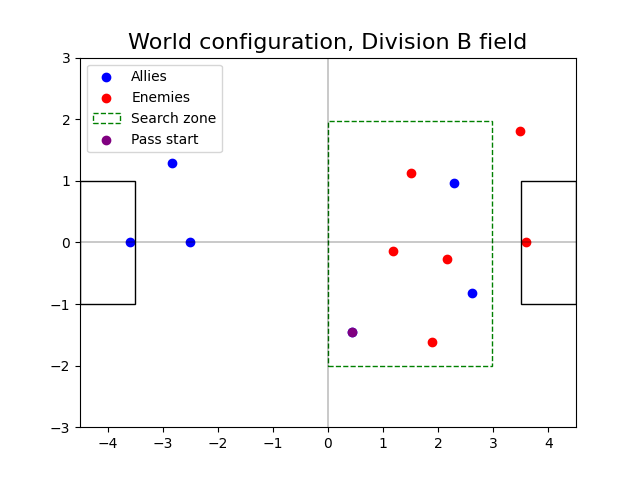
\includegraphics[scale=0.6]{world}
    \caption{Testing world configuration for the pass score estimation algorithm implemented. The red points are the enemies and
    is placed on the positive half of the field. Search grid has been limited inside the enemy's side. Allies are depicted in blue.}
    \label{fig:world-setup}
\end{figure}


By summing up these score computations, alongside a given weight for each $\sum{\omega_{i}s_i}$ with $\omega_i$ the weight for each $s_i$ score computed.
This allows us to tune the algorithm to favour certain conditions over others. Figure \ref{fig:combined} presents the resulting score heatmap obtained
on a given world configuration, with figure \ref{fig:world-setup}.

\begin{figure}[h]
    \centering
    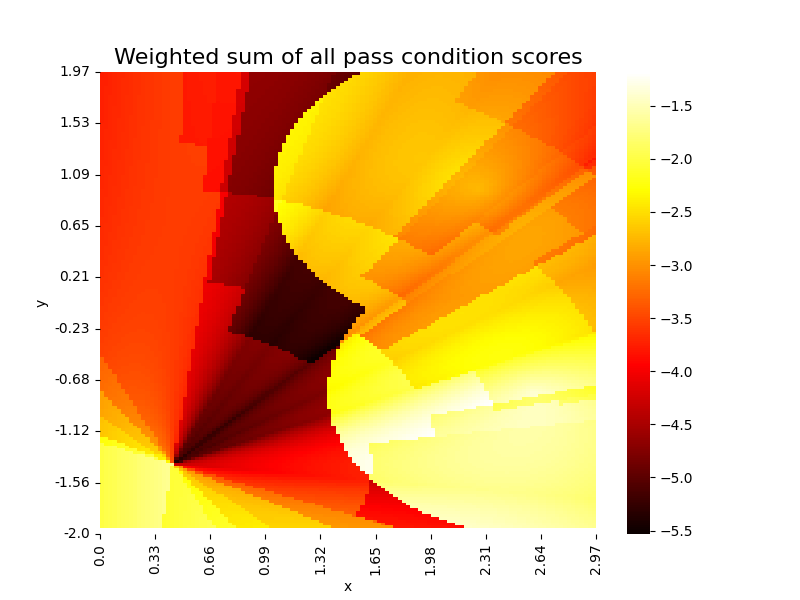
\includegraphics[scale=0.5]{combined}
    \caption{Resulting weighted sum for each point computed inside the search space. The heatmap is not smoothed
    and presents a value for each point. All weights of the score functions were set to one, with the exception of the ``closest ally'' condition,
    whose weight was set to 4.}
    \label{fig:combined}
\end{figure}
